\section{Introduction}

\begin{figure}
	\centering
	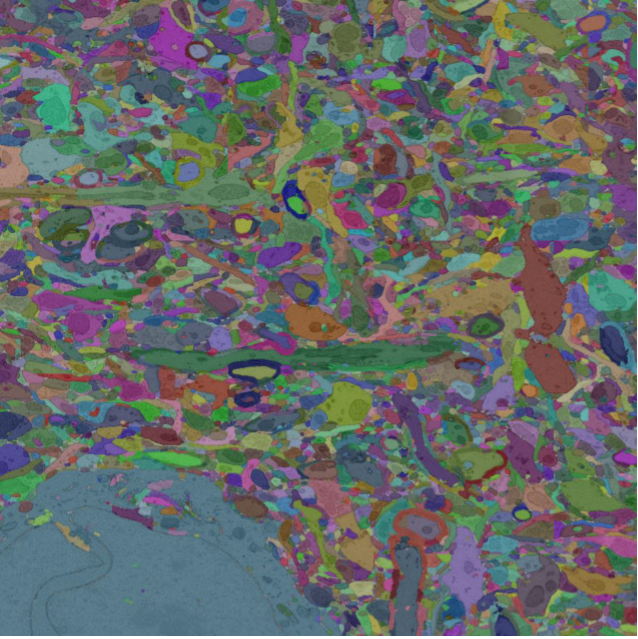
\includegraphics[width=0.42\linewidth]{./figures/intro-slice.png}
	\hspace{0.085\linewidth}
	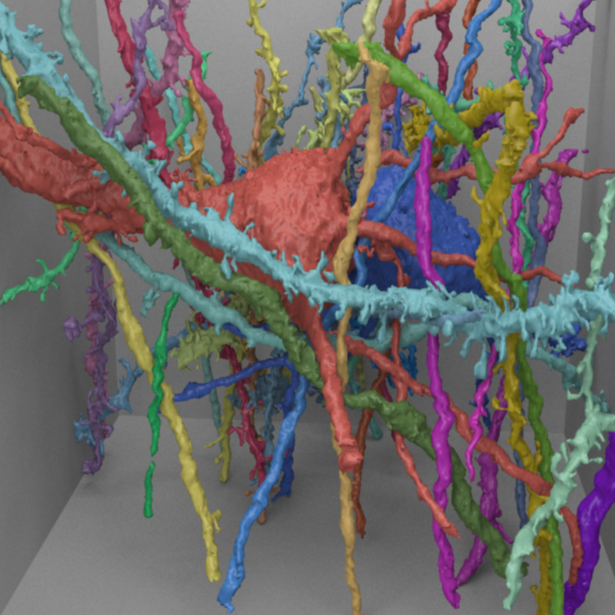
\includegraphics[width=0.42\linewidth]{./figures/intro-cube.png}
\end{figure}

Connectomics, the field of large-scale nanometer reconstruction of the wiring diagram of the brain, has created datasets petabytes in size. With recent advancements in image acquisition, neuroscientists are producing a terabyte of raw electron micronscopy image data every hour \cite{hildebrand2017whole}. Needless to say, it is impossible for domain experts to manually label this bulk of 3-D image data. However, many neuroscientists believe that they will be able to explore new insights into the workings of the brain by creating a complete wiring diagram of the brain \cite{kasthuri2015saturated}. These observations will create new advancements in neuromedicine, artificial intelligence, and (CITE). 

The access to significant datasets and potential for significant scientific contributions to the field of medicine has created a ripe environment for automatic reconstruction of these EM images. Significant research in the field has focused on extracting complete neuron reconstructions using the raw EM images. These techniques use only the image values acquired from the microscopes to agglomerate pixels into neuron predictions. Frequently, convolutional neural networks predict affinities between pixels \cite{ronneberger2015u,lee2015recursive}. 

Using only pixel data is not enough for full reconstruction of these datasets (CITE), and so researchers create a level of abstraction on top of the per-pixel algorithms. Under the new domain, researchers used these per-pixel algorithms as input to agglomerate pixels into super-pixels and create larger neuron reconstructions \cite{nunez2014graph} (CITE NEUROPROOF). These algorithms considered higher level information such as the boundary statistics between pixel regions and simple shape descriptors (CITE LASH).  These algorithms outperform the per-pixel methods from before but still do not fully leverage the wealth of information available.

Here we present another level of abstraction above the agglomeration strategies of the last few years. Our algorithms focus on the overarching shapes of the an oversegmented label volume to determine potential merge candidates. After identifying merge regions, we present a 3-D convolutional neural network to predict merges using only as input the shapes of the regions considered. Lastly, we build all of these techniques into a graph representation of the label volume. This enables us to enforce global constraints on the resulting segmentation that more closely match the biological principles. 